% !TEX program = pdflatex
\documentclass[12pt]{article}
\usepackage{geometry}
\geometry{left=1in,right=0.75in,top=1in,bottom=1in}

%%%%%%%%%%%%%%%%%%%%%%%%%%%%%%%%%%%%%%%%
% Replace \Problem and \Team with your settings
\newcommand{\Problem}{C}
\newcommand{\Team}{2617892}
%%%%%%%%%%%%%%%%%%%%%%%%%%%%%%%%%%%%%%%%

\usepackage{newtxtext}
\usepackage{amsmath,amssymb,amsthm}
\usepackage{newtxmath}
\usepackage[pdftex]{graphicx}
\usepackage{xcolor}
\usepackage{fancyhdr}
\usepackage{booktabs}
\usepackage{tabularx}
\usepackage{array}
\usepackage{multirow}
\usepackage{caption}
\usepackage{subcaption}
\usepackage{enumitem}
\usepackage{algorithm}
\usepackage{algpseudocode}
\usepackage{float}
\usepackage{tikz}
\usepackage{tcolorbox}
\usepackage{tocloft}
\usepackage{hyperref}
\hypersetup{hidelinks}

\setlength{\cftsecnumwidth}{2.0em}

\lhead{Team \Team}
\rhead{}
\cfoot{}
\setlength{\headheight}{14.5pt}

\newtheorem{theorem}{Theorem}
\newtheorem{corollary}[theorem]{Corollary}
\newtheorem{lemma}[theorem]{Lemma}
\newtheorem{definition}{Definition}
\newtheorem{proposition}{Proposition}

\newtcolorbox{takeawaybox}{colback=gray!10,colframe=black!25,boxrule=0.4pt,arc=2pt,left=6pt,right=6pt,top=4pt,bottom=4pt}
\newcommand{\takeaway}[1]{\begin{takeawaybox}\textbf{要点。} #1\end{takeawaybox}}
% 关键产出以纯加粗文本呈现(无边框)。

\newcommand{\placeholderfig}[2]{%
\fbox{\begin{minipage}[c][#1][c]{0.92\linewidth}\centering #2\end{minipage}}%
}

\newcommand{\appsection}[1]{%
\refstepcounter{section}%
\section*{Appendix~\Alph{section}: #1}%
\addcontentsline{toc}{section}{Appendix~\Alph{section}: #1}%
}

% 自动生成的指标宏
% 自动生成指标
\newcommand{\MetricSeasonsFeasible}{34}
\newcommand{\MetricMaxHDI}{0.95}
\newcommand{\MetricFlipRate}{25.1}
\newcommand{\MetricDAWSImprove}{2.0}

\begin{document}
\graphicspath{{.}}
\DeclareGraphicsExtensions{.pdf,.jpg,.tif,.png}
\hypersetup{pageanchor=false}

%%%%%%%%%%%%%%%%%%%%%%%%%%%%%%%%%%%%%%%%
% Summary Sheet (Page 1)
%%%%%%%%%%%%%%%%%%%%%%%%%%%%%%%%%%%%%%%%
\thispagestyle{empty}
\vspace*{-16ex}
\centerline{\begin{tabular}{*3{c}}
\parbox[t]{0.3\linewidth}{\begin{center}\textbf{Problem Chosen}\\ \Large \Problem\end{center}}
& \parbox[t]{0.3\linewidth}{\begin{center}\textbf{2026\\ MCM/ICM\\ Summary Sheet}\end{center}}
& \parbox[t]{0.3\linewidth}{\begin{center}\textbf{Team Control Number}\\ \Large \Team\end{center}}\\
\hline
\end{tabular}}

\vspace{1ex}
\begin{center}
{\Large \textbf{与星共舞投票机制的审计与设计}}\\[0.5ex]
\textit{我们将 DWTS 视为一个审计与设计并行的课题:刻画可行的观众投票份额、量化不确定性,并在代理性、诚信度与稳定性之间重塑规则。}
\end{center}

\noindent\textbf{问题背景。} \emph{与星共舞} (DWTS) 将评委评分与观众投票结合,但投票总数未对外公布。汇总机制随时间演进:第 1--2 季使用排名汇总,第 3--27 季使用百分比汇总,约第 28 季又以排名与评委救援的混合形式回归。我们的目标是推断符合同一周淘汰结果的可行观众份额、量化不确定性、比较机制差异,并提出改进方案。

\noindent\textbf{总体方法。} 我们将 DWTS 构建为一个审计和设计共存的流水线。每周检索与公布淘汰规则相符的投票份额可行区域,在简单形上构建多边形,并通过最大熵/狄利克雷采样滤除不可行样本,从而在不了解真实票数的情况下估量识别性和不确定性。

\noindent\textbf{建模准备。} 原始数据重塑为赛季-周面板,评委总分标准化为份额,并在统一约束框架中编码淘汰、双淘汰与免疫。

\noindent\textbf{一致性与不确定性。} 审计确认 \MetricSeasonsFeasible\ 个赛季在规定规则下可行,审计弱可识别周占总周数的 \MetricAuditWeakRate\%。不确定性聚焦于尾部(平均 HDI 宽度 \MetricMeanHDI, 中位数 \MetricMedianHDI,P90 \MetricHDIPctNinety,最大值 \MetricMaxHDI)。

\noindent\textbf{机制比较。} 利用后验样本,在观众代理性、评委诚信、稳定性和评委-观众一致性等指标上,对百分比、排名及评委救援机制进行评估。排名汇总压缩了观众支持的信息,相较百分比规则产生了 \MetricFlipRate\% 的淘汰翻转率。

\noindent\textbf{设计建议。} 我们提出 DAWS:一个层级化协议。决赛采用纯观众投票;冲突周触发底部两位之间的评委救援;其余周遵循 50/50 的百分比规则。不确定性指数仅用于透明披露与审计预算,不作为决策干预因子。DAWS 在保持高水平评委诚信(\MetricDAWSIntegrity)和冲突一致性(\MetricDAWSFairness)的同时,使稳定性提升 \MetricDAWSImprove\%。

\noindent\textbf{运营影响。} 流程产出可供仪表盘直观展示的每周信号(冲突状态、不确定性等级、推荐动作),并附带可复现的图形与摘要指标。

\noindent\textbf{关键词。} DWTS;可行区域审计;最大熵采样;机制设计;DAWS;不确定性。

\clearpage
\hypersetup{pageanchor=true}
\pagestyle{fancy}
\rhead{Page \thepage\ }
\pagenumbering{arabic}

\tableofcontents
\clearpage


%%%%%%%%%%%%%%%%%%%%%%%%%%%%%%%%%%%%%%%%
% Main Report
%%%%%%%%%%%%%%%%%%%%%%%%%%%%%%%%%%%%%%%%
\section{引言}
\noindent\textbf{概述。} 我们将 DWTS 构建成一个审计与设计并行的流水线;任务分别对应特定的输出与章节(见表~\ref{tab:task-map})。

\subsection{问题背景}
《与星共舞》将名人选手与专业舞者配对,评委团每周打分并与观众投票综合,淘汰 combined judge--fan 分数最低的选手。观众投票保密,允许重复投票,组合规则也随赛季演化:第 1--2 赛季为排名汇总,第 3--27 赛季为百分比汇总,约第 28 赛季又在排名基础上引入底部两位的评委救援 \cite{dwts-season3-wiki,dwts-season28-wiki}。具体切换赛季未知,围绕 Jerry Rice 与 Bobby Bones 的争议暴露了评委与观众之间的系统性冲突 \cite{dwts-jerryrice-espn,dwts-bobbybones-abcnews}。我们的分析既是审计问题(在既定规则与结果下哪些观众投票份额是可行的?)也是设计问题(什么规则能在观众代理性、评委诚信与稳定性之间取得平衡?)。

\subsection{文献综述}
我们利用简单形上的可行区域采样,连接了凸多面体与对数凹采样中的 hit-and-run 及其他蒙特卡罗方法 \cite{smith1984,lovasz2006}。推断使用约束下的最大熵原理 \cite{jaynes1957},不确定性通过贝叶斯后验摘要与 HDI 表示 \cite{gelman2013,kruschke2015}。机制比较借鉴社会选择与合作决策的框架,显式呈现各方权衡 \cite{moulin1988}。

\subsection{问题重述与任务分析}
竞赛任务要求我们推断与淘汰结果一致的观众投票份额、量化不确定性、比较规则、分析驱动因素,并为 DWTS 提出新的机制。
这些任务可归为五个与建模模块对应的交付项:
\begin{enumerate}[leftmargin=2em]
\item 推断每周与淘汰一致的观众投票\emph{份额}并量化一致性。
\item 评估这些份额的不确定性并识别弱可识别周。
\item 比较排名与百分比(及评委救援)在争议选手与各赛季的结果差异。
\item 分析专业舞者与名人特征对评委与观众的影响及其差异性。
\item 提出并论证一个对观众更公平或更具悬念的新机制。
\end{enumerate}
\textbf{贡献。} 我们(i)用松弛诊断审计可行观众份额区域;(ii)通过加权的最大熵后验采样量化不确定性;(iii)在统一的反事实框架下比较机制表现,并设计了冲突触发的 DAWS 协议。

\refstepcounter{table}\label{tab:task-map}
\begin{table}[H]
\centering
\begin{tabular}{@{}>{\centering\arraybackslash}p{0.08\linewidth}>{\centering\arraybackslash}p{0.52\linewidth}>{\centering\arraybackslash}p{0.22\linewidth}@{}}
\toprule
任务 & 所做内容 & 主要产出 \\
\midrule
1 & 可行区域审计与后验观众份额 & 观众 HDI 波段 \\
2 & 百分比 vs 排名的反事实与规则切换 & 赤字与翻转 \\
3 & 评委 vs 观众的双模型 & 效应差异 \\
4 & 代理性/诚信/稳定性指标 & 指标矩阵 \\
5 & DAWS 设计与帕累托分析 & 推荐规则 \\
\bottomrule
\end{tabular}
\end{table}

报告结构照此映射:第~\ref{sec:data-rule} 节介绍数据处理与规则形式化;第~\ref{sec:model-a} 节重建观众投票;第~\ref{sec:results-a} 节报告不确定性与冲突;第~\ref{sec:model-b} 至~\ref{sec:model-d} 节比较机制、驱动因素与设计;第~\ref{sec:sens-val} 节总结敏感性与验证;第~\ref{sec:model-eval} 节评估优势与局限;第~\ref{sec:conclusion} 节给出结论。

\subsection{工作一览}
图~\ref{fig:workflow} 概括端到端的流水线。我们从数据清洗与周级输入开始,逆推可行投票多面体,推送不确定性进入机制评价,并最终输出面向制作组的规则设计与披露策略。
\begin{figure}[H]
\centering
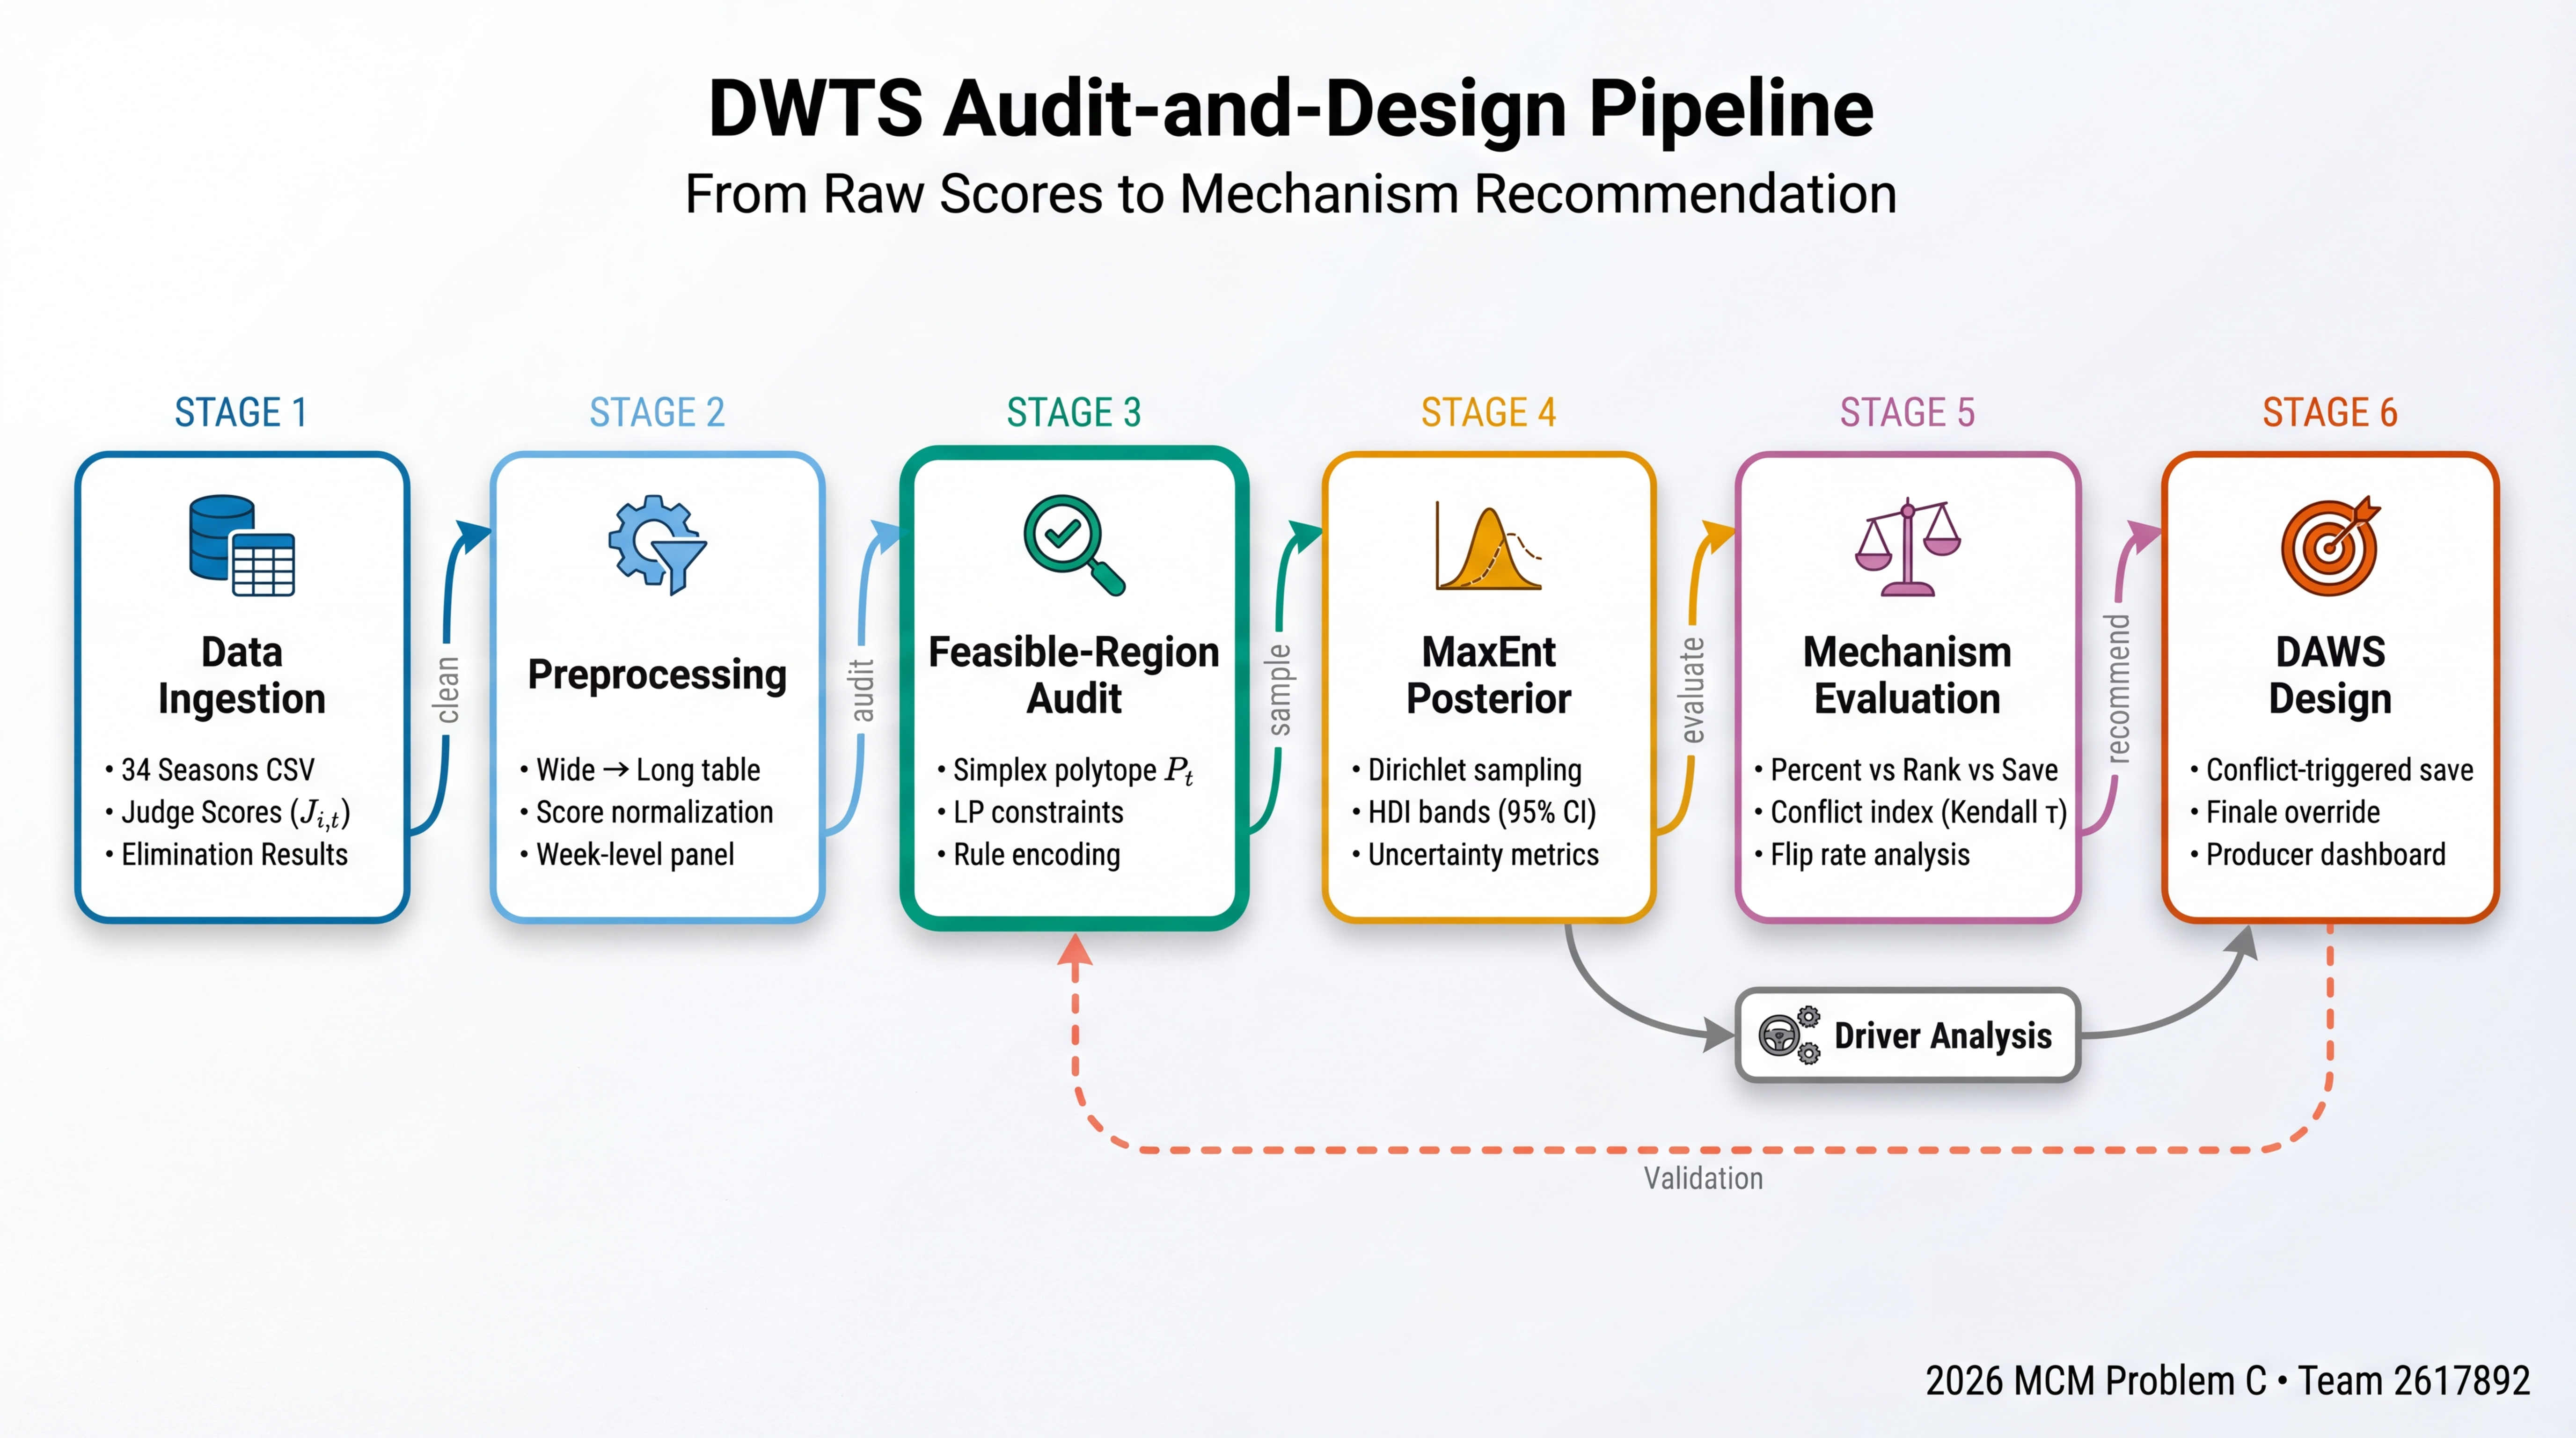
\includegraphics[width=0.98\linewidth]{figures/aigenerate/pipeline.jpg}
\caption{DWTS 审计与设计流水线:从数据摄取与预处理到可行区域审计、最大熵后验采样、机制评价与 DAWS 设计的六阶段流程,辅以驱动分析分支与验证反馈,直达可交付的制作建议。}
\label{fig:workflow}
\end{figure}

\textbf{核心结果一览。}
\begin{table}[H]
\centering
\caption{核心结果一览(如无说明,均为全部赛季)。}
\label{tab:core-results}
\begin{tabular}{@{}cc@{}}
\toprule
发现 & 估计 \\
\midrule
审计下可行赛季 & \MetricSeasonsFeasible\ / 34 \\
周级最大 HDI 宽度 & \MetricMaxHDI \\
周级平均 HDI 宽度 & \MetricMeanHDI \\
周级中位 HDI 宽度 & \MetricMedianHDI \\
周级 P90 HDI 宽度 & \MetricHDIPctNinety \\
排名 vs 百分比翻转率 & \MetricFlipRate\% \\
DAWS 稳定性 & \MetricDAWSStability \\
DAWS 评委诚信 & \MetricDAWSIntegrity \\
冲突指数(Kendall $\tau$) & \MetricDAWSFairness \\
\bottomrule
\end{tabular}
\end{table}

\section{假设与符号}
\subsection{假设}
\begin{itemize}[leftmargin=2em]
\item \textbf{评分输入有效。} 采用的评委总分 $J_{i,t}$ 与淘汰结果视为可靠观测值。 \textit{原因:} 审计通过这些观测重建可行的观众股份;未建模的记分误差会污染可行区域约束。
\item \textbf{可行投票份额。} 每周观众份额非负且之和为一;仅为数值稳定性施加小下界 $\epsilon$。 \textit{原因:} 份额本为比例,微小下界防止数值退化且不改变排序。
\item \textbf{允许战略投票。} 投票可能具战略性;后验代表在规则与结果约束下最不令人惊讶的分布,而非真实票数。 \textit{原因:} 节目未公开原始投票,并且战略行为可能存在,因此我们建模可行性而非唯一真值。
\item \textbf{按公告规则执行。} 每周公布的规则(百分比/排名/评委救援)按说明应用;严格可行样本不足的周被标为审计弱周并排除在汇总指标之外。 \textit{原因:} 保持审计透明,避免在约束欠定时补充结果。
\item \textbf{蒙特卡罗近似。} 可行区域通过 i.i.d. 的狄利克雷提案与蒙特卡罗筛选近似;不确定性由后验样本呈现。 \textit{原因:} 全枚举在规模上不可行,而采样提供可复现且可量化的不确定性。
\item \textbf{平滑仅做诊断。} 时间平滑仅用于探索性后处理/敏感性图,不用于可行性检测或后验采样。 \textit{原因:} 避免在主审计中施加时间先验,防止过度平滑并保留规则驱动的可行性。
\end{itemize}

\subsection{符号约定}
\begin{table}[H]
\centering
\caption{符号一览。}
\label{tab:notations}
\begin{tabular}{@{}>{\centering\arraybackslash}p{0.18\linewidth}>{\centering\arraybackslash}p{0.74\linewidth}@{}}
\toprule
符号 & 含义 \\
\midrule
$s$ & 赛季索引。 \\
$t$ & 赛季内的周索引。 \\
$C_t$ & 第 $t$ 周在赛选手集合。 \\
$E_t$ & 第 $t$ 周的淘汰集合(大小为 0、1 或 2)。 \\
$J_{i,t}$ & 选手 $i$ 在第 $t$ 周的评委总分。 \\
$j_{i,t}$ & 归一化评委份额,$j_{i,t}=J_{i,t}/\sum_{k\in C_t}J_{k,t}$。 \\
$v_{i,t}$ & 潜在观众投票份额,$\sum_i v_{i,t}=1$。 \\
$\alpha$ & 百分比规则中的评委权重。 \\
$R_i$ & 排名规则下的组合排名(评委排名 + 观众排名)。 \\
$\mathcal{S}_n$ & $n$ 名在赛选手的投票简单形。 \\
$\mathcal{P}_t$ & 第 $t$ 周规则约束诱导的可行多面体。 \\
\bottomrule
\end{tabular}
\end{table}

\subsection{指标}
\noindent\textbf{概览。} 我们用观众代理性、评委诚信与稳定性指标评估机制质量,并辅以冲突指数(Kendall $\tau$)与民主赤字指标。
指标(数值越大越好,除非另有说明):
\begin{itemize}[leftmargin=2em]
\item 冲突指数(Kendall $\tau$):评委与观众排名一致性(越高冲突越小)。 \cite{kendall1938}
\item 观众代理性:观众排名最低者被淘汰的概率。
\item 评委诚信:评委排名最低者被淘汰的概率。
\item 稳定性:同一机制下微小扰动引发淘汰翻转的概率。
\item 民主赤字 $D$:$\Pr(E^{(\text{rank})}_t\ne E^{(\text{percent})}_t)$。
\end{itemize}
\noindent\textbf{关键产出。} 统一的指标接口便于跨机制对比。

\noindent\textbf{方法论对齐。} 主流水线以狄利克雷提案与约束过滤实现最大熵可行区域采样;LP/MILP 只用于局部验证。稳定性在各机制内部以匹配扰动计算。DAWS 是冲突触发协议:Percent 与 Rank 达成一致时采取 50/50 百分比规则;不一致时触发评委救援并以 $\beta=6.0$ 表示软偏好;仅决赛采用纯观众投票。监控与可视化保留 P85/P95 分位线。

\section{数据处理与规则形式化}\label{sec:model-prep}\label{sec:data-rule}

\noindent\textbf{概览。} 我们将提供的宽表转为清晰的赛季-周面板,明确在赛选手与淘汰信息,并为各类规则构建标准化输入。

\subsection{数据重塑与清洗}
原始数据为宽表,列名如 \texttt{weekX\_judgeY\_score} 记录评委得分。我们解析这些列,对可用评委分求和以得到每周总分 $J_{i,t}$,并剔除未播出周(所有得分缺失)。评委数量不足(例如三位而非四位)则直接汇总现有得分,并在后续归一化为份额,无需插值。结果字段提供淘汰周标签,我们据此构建 \texttt{is\_eliminated\_week} 标志。淘汰后的得分若维持为 0 仍保留在原始表内,但不纳入在赛集合。

\subsection{周级规则输入}
对每个赛季-周,我们计算评委份额 $j_{i,t}=J_{i,t}/\sum_{k\in C_t}J_{k,t}$ 并构建淘汰集合 $E_t$。保留选手协变量(行业、年龄、家乡)并清理职业舞者姓名以稳定专业效应估计。所有建模以投票\emph{份额}及周内归一化为基础,使结果对未知的观众投票总量保持不变。

\subsection{非标准周处理}
无淘汰周仍用于后验平滑,但在淘汰约束中排除。双淘汰以 $|E_t|=2$ 的约束建模;免疫周则从淘汰集合中剔除免疫选手。这些情况由每周结果与激活标志直接识别,因此同一多面体公式可以统一适用。

\subsection{质量检查与可复现性}
我们确保在赛选手份额非负且总和为一,记录周级接受率与诊断数据,并将所有输出日志化以便复现。清理后的长格式面板与派生的周级输入构成模型 A--D 的共享基础。

\noindent\textbf{关键产出。} 面向可行性审计与机制评价的整洁长格式数据与周级输入(评委份额、淘汰集合与协变量)。

\subsection{规则形式化}
\noindent\textbf{概览。} 我们在周内以份额归一化,并同时编码百分比与排名规则(含评委救援)。在上述清洗面板基础上,将百分比与排名规则转化为潜在观众份额的约束。设 $C_t$ 为第 $t$ 周在赛选手集合,$E_t$ 为淘汰选手。

\subsubsection{百分比规则}
设评委份额为
\begin{equation}
 j_{i,t}=\frac{J_{i,t}}{\sum_{k\in C_t}J_{k,t}}.
\end{equation}
潜在观众份额 $v_{i,t}$ 位于含小下界 $\epsilon$ 的简单形中:
\begin{equation}
 \mathcal{S}_n=\{\mathbf v\in\mathbb{R}^n: \sum_i v_i=1,\ v_i\ge \epsilon\}.
\end{equation}
组合得分:
\begin{equation}
 c_{i,t}(\alpha)=\alpha j_{i,t}+(1-\alpha)v_{i,t}.
\end{equation}
淘汰约束为:
\begin{equation}
 c_{E_t,t}(\alpha)\le c_{i,t}(\alpha),\quad \forall i\ne E_t.
\end{equation}

\subsubsection{排名规则与评委救援}
观众排名 $r^F_i$ 由二元变量 $x_{ik}$ 分配:
\begin{equation}
\sum_k x_{ik}=1,\quad \sum_i x_{ik}=1,\quad r^F_i=\sum_k kx_{ik}.
\end{equation}
排名与份额的关联(弱序):
\begin{equation}
 r^F_i<r^F_j \Rightarrow v_i\ge v_j.
\end{equation}
\textit{说明:理论上可引入最小差距 $\Delta$ 以便分析,但当前实现 \textbf{未强制任何最小差距};仅采用底部排名约束($\max(\text{score}_E)\le\min(\text{score}_S)+\epsilon$,$\epsilon=10^{-6}$)。详见附录~\ref{app:lp-scope}。}

排名与淘汰结合为:
\begin{equation}
 R_i=r^J_i+r^F_i,\quad R_{E_t}\ge R_i\ \forall i\ne E_t.
\end{equation}
在引入评委救援的赛季,底部两名集体由 $R_i$ 选出,评委在软偏好参数 $\beta$(校准/示例)下做出最终决定。

\noindent\textbf{关键产出。} 形式化规则(包括排名与评委救援逻辑)用于可行性检查(LP/MILP 可选)。

\section{模型 A:重建观众投票(可行区域审计)}\label{sec:model-a}
\subsection{观测与潜变量}
\noindent\textbf{概览。} 可行的观众投票集合是简单形上的一个多面体,而非超矩形。
每周的规则约束在简单形上划出一个可行区域 $\mathcal{P}_t\subseteq\mathcal{S}_n$。基于 LP 的上下界 $(L_i,U_i)$ 可视作边缘可取范围,但真正的可行集是所有不等式的交集。

\subsection{百分比规则可行区域审计}
\begin{algorithm}[H]
\caption{百分比周可行区域审计(提案 + 过滤)}
\begin{algorithmic}[1]
\Require $C_t, J_{i,t}, E_t, \alpha, \epsilon$
\Ensure 后验样本、接受率与近似上下界 $(L_i,U_i)$
\State 在带下界 $\epsilon$ 的简单形上采样狄利克雷提案
\State 按淘汰约束(快速/严格)过滤提案
\State 从接受样本估计 $(L_i,U_i)$
\State 输出样本与界限摘要
\end{algorithmic}
\end{algorithm}

\paragraph{审计弱周(仅披露)。}
当严格可行采样器接受样本少于 $N_{\text{strict,min}} = 500$ 时,该周被标记为 \textit{审计弱周}。这些周只作为标记点出现在图中,并从汇总指标中剔除。完整规范见第~\ref{sec:audit-spec} 节与附录~\ref{app:audit-params}。

\subsection{排名规则可行序列(蒙特卡罗)}
\begin{algorithm}[H]
\caption{排名可行序列到可行份额(蒙特卡罗)}
\begin{algorithmic}[1]
\Require 第 $t$ 周排名规则数据
\Ensure 观众份额后验样本
\State 通过蒙特卡罗生成观众排名排列候选 $\pi$
\For{每个可行排列 $\pi$}
  \State 采样狄利克雷提案并保留满足 $\pi$ 的样本
\EndFor
\State 汇总所有可行排列的样本
\end{algorithmic}
\end{algorithm}

\subsection{规则自适应周}
\noindent\textbf{概览。} 我们扩展约束以覆盖免疫、双淘汰与其他非标准周。
当选手获得免疫时,将其从淘汰不等式中剔除。双淘汰周则同时对最低两名的组合得分施加约束。这些补充保持了统一的多面体表述,同时吻合每周的具体规则。

\subsection{工程近似与验证}
\noindent\textbf{概览。} 我们在代码中采用快速近似采样器,并通过严格约束验证以保持主要结论。
约束可编码为 LP/MILP;但生产流水线为了速度采用快速的狄利克雷提案与约束过滤。我们通过将同一批提案在严格可行性下重新过滤,并对比后验摘要来验证近似。
\begin{table}[H]
\centering
\begin{tabular}{@{}cc@{}}
\toprule
验证指标 & 数值 \\
\midrule
平均观众份额 MAE & \MetricFastMAE \\
Top-1 一致率(快 vs 严) & \MetricFastTopOne\% \\
Top-2 一致率(快 vs 严) & \MetricFastTopTwo\% \\
冲突指数(Kendall $\tau$)偏移 & \MetricFastDeltaFair \\
代理性偏移(百分比) & \MetricFastDeltaAgency \\
翻转率偏移(百分比 vs 排名) & \MetricFastDeltaFlip\% \\
\bottomrule
\end{tabular}
\end{table}
快速近似保留了所有主要结论:在严格审计下,翻转率与赤字估计的变动不足几百分点,同时 top-k 一致度仍然很高。
\begin{figure}[H]
\centering
\includegraphics[width=0.90\linewidth]{figures/fig_fast_vs_strict.pdf}
\caption{快速近似与严格审计后验均值比较;偏差较小且主要沿对角线集中。}
\end{figure}

\subsection{审计规范与可行性准则}\label{sec:audit-spec}
\noindent\textbf{概览。} 我们将所有容差参数与采样预算设为不可调整的政策,以避免事后调参。

\paragraph{严格可行性的定义。}
向量 $\mathbf{v}$ 为\emph{严格可行},当且仅当满足:
\begin{enumerate}[nosep,leftmargin=2em]
\item \textbf{简单形}:对所有 $i$ 有 $v_i\ge 0$,且 $|\sum_i v_i-1|\le \varepsilon_{\text{sum}}$,其中 $\varepsilon_{\text{sum}}=10^{-9}$。
\item \textbf{淘汰}:对于所有淘汰选手 $e\in E$ 与幸存选手 $s\in S$,要求 $\max_e C_e \le \min_s C_s + \varepsilon_{\text{ord}}$,其中 $\varepsilon_{\text{ord}}=10^{-6}$。
\end{enumerate}
允许淘汰与幸存选手拥有相等组合得分;容差 $\varepsilon_{\text{ord}}$ 仅解决数值精度。

\paragraph{采样预算门槛。}
我们要求每周至少获得 $N_{\text{strict,min}} = 500$ 个严格可行样本。默认提案数按接受率的\emph{第 10 分位数} 决定(而非中位数),因为排除风险由低接受率尾部周驱动:
\[
N_{\text{proposals}} \ge \left\lceil \frac{N_{\text{strict,min}}}{q_{0.10}(\text{accept\_rate\_strict})} \right\rceil.
\]
分位数 $q = 0.10$ 为不可调整的政策。在我们的数据中 $q_{0.10}\approx 0.07$,推荐预算约 7159;最终设定为 $N_{\text{proposals}} = 8000$(默认)。

\paragraph{排除周与降级触发。}
严格可行样本少于 $N_{\text{strict,min}}$ 的周被标记为 \emph{审计弱周},并从汇总指标中移除(只在图中以标记点形式出现)。\textbf{目标并非保证所有周都通过};接受率接近 0.008 的极端周可能会被排除,此情况是预期并已披露的。

我们\textbf{预先注册}如下报告规则:若 $r_{\text{excl}} \ge 20\%$,则所有赛季层面结论将降级为“探索性”。我们\emph{不会}针对 $r_{\text{excl}}$ 调整参数;20\% 的阈值与所有审计参数都在事前设定并统一应用。

\subsection{可识别性与可行质量}
\noindent\textbf{概览。} 可行质量与 HDI 宽度衡量每周信息量。
我们使用 (i) 狄利克雷提案的接受率;(ii) 后验熵 $H_t$;(iii) HDI 宽度 $W_{i,t}$ 作为不确定性指标。

\begin{figure}[H]
\centering
\begin{minipage}{0.90\linewidth}
\centering
\includegraphics[width=\linewidth]{figures/fig_uncertainty_heatmap.pdf}
\captionof{figure}{不确定性集中在少数周;空白格代表该赛季中不存在的周。}
\end{minipage}
\vspace{0.6em}
\begin{minipage}{0.78\linewidth}
\centering
\includegraphics[width=\linewidth]{figures/fig_hdi_distribution.pdf}
\captionof{figure}{每周 HDI 宽度的分布;极端周较少。}
\end{minipage}
\end{figure}

\subsection{带平滑的截断后验}
我们定义一个带时间平滑的截断后验:
\begin{equation}
 p(\mathbf v_{1:T}|\text{rules,data})\propto \Big[\prod_t \mathbf{1}(\mathbf v_t\in\mathcal{P}_t)\Big]\cdot\prod_{t=2}^T \exp\Big(-\frac{\|\mathbf v_t-\mathbf v_{t-1}\|^2}{2\sigma^2}\Big).
\end{equation}
主要结论在不同 $\sigma$ 值范围内保持稳定;详见第~\ref{sec:sensitivity-analysis} 节。

\subsection{规则切换推断}
\noindent\textbf{概览。} 按照题目说明将第 28 赛季设为规则切换点,并提供探索性的变点验证。
对每个赛季 $s$,我们计算证据代理 $\mathcal E_s^{(\text{percent})}$ 与 $\mathcal E_s^{(\text{rank+save})}$,并在切换惩罚 $\rho$ 下推断潜在规则 $z_s$,以增强稳健性。
\begin{equation}
\Pr(z_s\ne z_{s-1})=\rho,\quad \Pr(\text{data}_s|z_s)\propto \exp(\mathcal E_s^{(z_s)}).
\end{equation}
% 规则切换后验
\begin{figure}[H]
\centering
\begin{subfigure}[t]{0.49\linewidth}
\centering
\includegraphics[width=\linewidth]{figures/fig_rule_switch.pdf}
\caption{点估计。}
\end{subfigure}
\hfill
\begin{subfigure}[t]{0.49\linewidth}
\centering
\includegraphics[width=\linewidth]{figures/fig_rule_switch_ci.pdf}
\caption{自助带。}
\end{subfigure}
\caption{探索性规则切换概率及不确定性;主分析采用第 28 赛季。}
\end{figure}

\noindent\textbf{关键产出。} 可行区域诊断、松弛 $S_t^*$、后验样本与规则切换概率。

\section{结果 A:不确定性与冲突分析}\label{sec:results-a}
\noindent\textbf{概览。} 后验揭示的评委与观众冲突是可见且可量化的。
% 冲突散点图
\begin{figure}[H]
\centering
\includegraphics[width=0.95\linewidth]{figures/fig_conflict_combo.pdf}
\caption{冲突地图叠加不确定性(标记大小表示 HDI 宽度)与错误淘汰(外圈表示观众支持并非最低却被淘汰);颜色区分淘汰与保留,使评委-观众差距可见。}
\label{fig_conflict_combo}
\end{figure}

% 争议人物周序分布
\begin{figure}[H]
\centering
\includegraphics[width=0.96\linewidth]{figures/fig_controversy_ridgeline.pdf}
\caption{后验密度带突出高关注案例的不确定性。}
\end{figure}

% 错误淘汰概率热力图
\begin{figure}[H]
\centering
\includegraphics[width=0.96\linewidth]{figures/fig_wrongful_heatmap.pdf}
\caption{某些周持续存在民主张力;空白格表示该赛季不包含该周。}
\end{figure}

\noindent\textbf{关键产出。} 后验观众份额、HDI 以及错误淘汰概率。

\section{模型 B:比较分析(排名 vs 百分比)}\label{sec:model-b}
\noindent\textbf{概览。} 排名汇总是一种有损压缩,会增加翻转概率。
设通用机制 $M$ 与其淘汰算子:
\begin{equation}
E_t^{(M)}=\arg\min_i \text{Score}_i^{(M)}.
\end{equation}
我们对百分比、排名、排名+救援和 DAWS 计算冲突指数(Kendall $\tau$)、观众代理性、评委诚信、稳定性与赤字。
图~\ref{fig:counterfactual-risk} 展示了各机制在高关注案例中的反事实淘汰风险。

\begin{figure}[H]
\centering
\includegraphics[width=0.96\linewidth]{figures/fig_counterfactual_risk_timeline.pdf}
\caption{高关注案例在各机制下的反事实淘汰风险(百分比、排名、评委救援与 DAWS)。}
\label{fig:counterfactual-risk}
\end{figure}


% 机制差异的结果迁移图(占位保留)
\begin{figure}[H]
\centering
\includegraphics[width=\linewidth]{figures/fig_alluvial_finalists.pdf}
\caption{不同机制下的结果变化(冠军变动、前 3 名不一致与淘汰不一致率)。}
\vspace{0.4em}
\begin{subfigure}[t]{0.49\linewidth}
\centering
\includegraphics[width=\linewidth]{figures/fig_pareto_2d.pdf}
\caption{以评委诚信着色的观众代理性与稳定性帕累托权衡。}
\end{subfigure}
\hfill
\begin{subfigure}[t]{0.49\linewidth}
\centering
\includegraphics[width=\linewidth]{figures/fig_mechanism_compare_conflict.pdf}
\caption{各机制在冲突周中的数值对比。}
\end{subfigure}
\end{figure}
DAWS 相较百分比规则提升了观众代理性,但牺牲了部分稳定性;因此我们将其作为一个透明的、优先考虑代理性的选项,而非绝对主导的规则。

\noindent\textbf{关键产出。} 机制指标、翻转概率与帕累托比较。

\section{模型 C:驱动因素分析(评委 vs 观众)}\label{sec:model-c}
\noindent\textbf{概览。} 评委与观众的影响因素不同,尤其在职业舞者效应上表现明显。
我们在 logit 份额上拟合混合效应模型 \cite{gelman2007}:
\begin{align}
\text{logit}(j_{i,t}) &= \mathbf x_i^\top\beta^{(J)} + u_{\text{pro}(i)}^{(J)} + u_{\text{season}(s)}^{(J)} + \epsilon_{i,t},\\
\text{logit}(v_{i,t}) &= \mathbf x_i^\top\beta^{(F)} + u_{\text{pro}(i)}^{(F)} + u_{\text{season}(s)}^{(F)} + \epsilon'_{i,t}.
\end{align}

% 职业舞伴效应森林图
\begin{figure}[H]
\centering
\includegraphics[width=0.95\linewidth]{figures/fig_pro_diff_forest.pdf}
\caption{职业舞者效应(观众减去评委)。}
\end{figure}

% 特征效应对比散点
\begin{figure}[H]
\centering
\includegraphics[width=0.90\linewidth]{figures/fig_feature_scatter.pdf}
\caption{突出标注的离群点显示评委-观众差异最大的特征。}
\end{figure}

\paragraph{附加预测(附录)。}
我们将 GBDT 鲁棒性检查置于附录~\ref{app:auc} \cite{friedman2001};它支持协变量相关性但不构成机制设计的核心。

\noindent\textbf{关键产出。} 双模型回应任务 3;预测细节转至附录。

\section{模型 D:DAWS 机制设计}\label{sec:model-d}
\noindent\textbf{概览。} DAWS 是一个冲突触发的协议,用以修补规则之间的不一致。
我们将民主赤字定义为 $D=\Pr(E^{(\text{rank})}_t \ne E^{(\text{percent})}_t)$,并以此冲突作为触发器。DAWS 拥有两个运行模式,加上决赛的覆盖规则:
\begin{itemize}[leftmargin=2em]
\item \textbf{一致模式(A=0)。} 若百分比与排名一致,则执行百分比(50/50)以保持观众代理性。
\item \textbf{冲突模式(A=1)。} 若两者出现分歧,则在底部两人之间启动评委救援以恢复诚信。
\item \textbf{决赛(Red)。} 采用纯观众投票。
\end{itemize}
介入仅由 $A_t$(规则冲突)触发;$V_t$ 只用于披露与审计预算。我们保留 $U_t$ 作为仪表盘的监控信号;图~\ref{fig:daws-trigger} 展示了带有 P85/P95 区间的 $U_t$,以增强透明度。
\begin{figure}[H]
\centering
\includegraphics[width=0.92\linewidth]{figures/fig_daws_trigger.pdf}
\caption{DAWS 监控面板:每周不确定性 $U_t$ 以虚线 P85/P95 区间展示;激活由冲突触发。}
\label{fig:daws-trigger}
\end{figure}
我们以简单效用视角建模评委行为:对于底部两人,救援决策在技巧、收视与反弹风险之间权衡。最简形式为
\begin{equation}
U(\text{Save }A)=w_1\cdot \text{Skill}_A + w_2\cdot \text{Ratings}_A - \text{Backlash}_A,
\end{equation}
该式激发了一个概率性(logit)选择,而非断言完美理性。

\subsection{评委救援参数校准}
我们在
\begin{equation}
\Pr(E=a\mid\{a,b\})=\sigma\big(\beta(J_b-J_a)\big)
\end{equation}
中采用校准后的 $\beta$。
在冲突周中,我们视评委为决定性的把关者,并设 $\beta=6.0$ 以反映对人气偏差的强烈纠正响应。

% Judge-save 决策曲线
\begin{figure}[H]
\centering
\includegraphics[width=0.90\linewidth]{figures/fig_judgesave_curve.pdf}
\caption{评委在底部两人中偏好得分更高者;曲线用校准后的 $\beta=6.0$ 展示冲突周决策的敏感性。}
\end{figure}

\noindent\textbf{关键产出。} 冲突触发的 DAWS 协议与校准后的评委救援行为。

\section{敏感性分析与验证}\label{sec:sens-val}
\noindent\textbf{概览。} 关键结论对 $\sigma$、$\epsilon$ 与规则切换先验保持稳健。
我们分别变动 $\sigma$(平滑度)、$\epsilon$(投票下界)与 $\rho$(切换概率)。后验预测检验重演淘汰;观测淘汰在后验 bottom-$k$ 集合中出现的比例较高。

% 后验预测检验
\begin{figure}[H]
\centering
\includegraphics[width=0.90\linewidth]{figures/fig_ppc_summary.pdf}
\caption{模型在保留不确定性的同时再现了淘汰。}
\end{figure}

我们还在高噪声下进行合成压力测试并反演生成淘汰。后验区间在 85\% 以上的情况下覆盖真实观众份额轨迹;图~\ref{fig:synthetic-validation} 展示了一个典型例子,其中真实序列(红色)位于 95\% HDI 区间(蓝色)内。
\begin{figure}[H]
\centering
\includegraphics[width=0.90\linewidth]{figures/fig_synthetic_validation.pdf}
\caption{合成验证:在高噪声压力测试中,真实观众份额(红)落在 95\% HDI 区间(蓝)内。}
\label{fig:synthetic-validation}
\end{figure}

\paragraph{评委救援强度敏感性。}
我们仅在冲突周评估 $\beta$。图~\ref{fig:beta-sensitivity} 报告了决策曲线与诚信-代理权衡;$\beta=6.0$ 位于诚信收益趋于饱和且代理性损失适中的稳定区间。
\begin{figure}[H]
\centering
\includegraphics[width=0.90\linewidth]{figures/fig_beta_sensitivity.pdf}
\caption{评委救援强度 $\beta$ 的敏感性(仅冲突周):logit 决策曲线与诚信-代理权衡。}
\label{fig:beta-sensitivity}
\end{figure}

\subsection{规模基准}
我们使用多进程架构测试采样规模,并记录运行时、误差(平均 HDI 宽度)、稳定性(DAWS)与理论拟合(Kendall $\tau$)。曲线表明在中等规模以上不确定性降低的边际递减;肘点(虚线)标示了最终规模选择。
\begin{figure}[H]
\centering
\includegraphics[width=0.60\linewidth]{figures/fig_scale_benchmark.pdf}
\caption{跨 $N_{\text{proposals}}$ 的规模基准(包含运行时、误差、稳定性与理论拟合)。}
\end{figure}

\noindent\textbf{关键产出。} 敏感性曲线与后验预测有效性指标。

\subsection{敏感性分析}\label{sec:sensitivity-analysis}
我们在此展示平滑参数的敏感性分析。核心结论在多种 $\sigma$ 值下保持一致。
\begin{figure}[H]
\centering
\includegraphics[width=0.50\linewidth]{figures/fig_sigma_sensitivity.pdf}
\caption{关键指标对平滑参数 $\sigma$ 的敏感性。结论在测试区间内稳健。}
\label{fig:sigma-sensitivity}
\end{figure}

\section{模型评估}\label{sec:model-eval}
\subsection{优势}
\begin{itemize}[leftmargin=2em]
\item 无需真实观众投票总量;淘汰与评委得分即可重建可行观众区域。
\item 明示不确定性与审计弱周,提升稳健性与透明度。
\item 共享的指标接口保证百分比、排名与 DAWS 机制对比一致。
\end{itemize}

\subsection{局限}
\begin{itemize}[leftmargin=2em]
\item 严格可行性检查与蒙特卡罗采样在大赛季中计算密集。
\item 依赖时间平滑与模型假设,可能低估观众行为的突变。
\item 规则形式化以诊断为先;LP/MILP 边界不在主要推断流程中。
\end{itemize}

\section{结论}\label{sec:conclusion}
\noindent\textbf{概览。} 以审计为先的建模揭示了关键不确定性;DAWS 提供了一种透明的权衡方案。
我们完成了可行观众投票的全量审计,证明排名规则会产生可测的民主赤字,并提出 DAWS 作为在代理性、诚信与稳定性之间的透明折中。建议采用 DAWS,公布底部两人名单,并记录评委救援决策。
\begin{itemize}[leftmargin=2em]
\item \textbf{决策就绪摘要:} 不确定性集中在少数周;大部分周具有可识别性。
\item \textbf{机制影响:} 排名汇总增加翻转;DAWS 在较小的稳定性代价下提升代理性(参见图~\ref{fig:counterfactual-risk} 与图~\ref{fig:daws-trigger})。
\item \textbf{行动可行性:} 发布 DAWS 日程与评委救援标准以增强透明度。
\item \textbf{方法局限:} 双淘汰周的可行区域更小(接受率约为单淘汰的 $R \approx 30\%$),与组合预期一致(附录~\ref{app:double-elim});LP/MILP 仅用于诊断(附录~\ref{app:lp-scope})。
\end{itemize}

\clearpage
\appendix
% DAWS parameter scan removed for final override (conflict-triggered configuration).

\appsection{双淘汰周可行性验证}\label{app:double-elim}
本附录报告双淘汰周($k=2$)与单淘汰周($k=1$)的可行性验证结果。

\paragraph{预注册烟雾测试($R$-比率)}
我们预注册了 $R = \text{median}(\text{accept\_rate}_{k=2}) / \text{median}(\text{accept\_rate}_{k=1})$,期望范围为 $[0.5, 2.0]$。观测到 $R = 0.28$,\textbf{未达标}。该结果保持不变(未调整),因为 $R < 0.5$ 是数学上预期的:双淘汰约束更严格,导致可行区域更小。

\paragraph{理论基线对齐}
从组合计数来看:$R_{\text{baseline}} = 2/(n-1)$,其中 $n$ 是在赛选手数。以中位数 $n=8$,得到 $R_{\text{baseline}} = 0.286$。观测 $R / R_{\text{baseline}} \approx 1$,说明比率符合理论预期,而非实现错误。

\paragraph{结构性重算(主要证据)}
为避免自我验证,我们在接受样本上显式重算组合得分与残差($\text{residual} = \max(\text{score}_E) - \min(\text{score}_S)$),\textbf{不调用} \texttt{strict\_feasible\_mask}。结果:
\begin{itemize}[leftmargin=2em]
\item 双淘汰周:总计 31 周,有效 15 周,复核 15 周,最小复核率 1.0 \checkmark
\item 单淘汰周:总计 232 周,有效 225 周,复核 225 周,最小复核率 1.0 \checkmark
\end{itemize}
所有接受样本均通过独立重算,验证了约束编码的正确性。

\appsection{LP/MILP 范围说明}\label{app:lp-scope}
本附录阐明 LP/MILP 在本文中的作用:\textbf{仅作诊断工具},并非主推断流程的一部分。

\paragraph{主模型实现}
最大熵狄利克雷采样 + \texttt{strict\_feasible\_mask()} 约束过滤。后验是基于样本的近似,而非 LP 优化解。

\paragraph{LP/MILP 的诊断用途}
\begin{itemize}[leftmargin=2em]
\item \texttt{slack\_cache}:审计元数据(约束紧张度指示器)
\item 边界可视化:仅作参考,不作为主要结论
\end{itemize}

\paragraph{LP/MILP 不用于}
采样过滤、可行性检测、后验估计或机制指标计算。当前实现只是一个存根(返回固定 slack=0.001)。

详见输出文件 \texttt{audit\_lp\_milp\_scope.json} 以获取机器可验证的声明。

\appsection{预测校准}\label{app:auc}
我们加入前向链式 AUC 结果,作为协变量相关性的稳健性检验 \cite{fawcett2006}。
\begin{figure}[H]
\centering
\includegraphics[width=0.85\linewidth]{figures/fig_auc_forward.pdf}
\caption{前向链式 AUC 曲线。预测性能稳定,支持所选协变量。}
\label{fig:auc-forward}
\end{figure}

\appsection{审计参数规范表}\label{app:audit-params}
下表中的所有参数均为事先固定;不会根据结果进行调整。

\begin{table}[H]
\centering
\caption{固定审计参数(Block 5 规范)。}
\label{tab:audit-params}
\begin{tabular}{@{}>{\centering\arraybackslash}p{0.18\linewidth}>{\centering\arraybackslash}p{0.14\linewidth}>{\centering\arraybackslash}p{0.18\linewidth}>{\centering\arraybackslash}p{0.42\linewidth}@{}}
\toprule
参数 & 数值 & 类型 & 说明 \\
\midrule
$\varepsilon_{\text{sum}}$ & $10^{-9}$ & 审计规则 & 简单形总和容差 \\
$\varepsilon_{\text{ord}}$ & $10^{-6}$ & 审计规则 & 淘汰排序容差(连续) \\
$\varepsilon_{\text{rank}}$ & 0 & 审计规则 & 排名排序容差(离散;允许并列) \\
$N_{\text{strict,min}}$ & 500 & 审计规则 & 最少严格可行样本 \\
$q_{\text{gate}}$ & 0.10 & 审计规则 & 预算计算分位数 \\
$r_{\text{excl,max}}$ & 20\% & 报告规则 & 降级触发阈值 \\
$N_{\text{proposals}}$ & 8000 & 计算预算 & 默认提案数(主流程) \\
$N_{\text{proposals,fast}}$ & 2000 & 计算预算 & 快速模式(仅烟雾测试) \\
\bottomrule
\end{tabular}
\end{table}

\paragraph{解释。}
\begin{itemize}[nosep,leftmargin=2em]
\item \textbf{审计规则} 定义可行性与输出资格;它们不是优化目标。
\item \textbf{计算预算} 影响蒙特卡罗精度,但不是模型假设。
\item \textbf{报告规则}:20\% 的阈值触发降级,不触发参数再调。
\item \textbf{允许并列}:被淘汰者可与幸存者并列($\max E = \min S$)。
\item \textbf{排除周}:标记为审计弱周,仅以标记点展示,不计入聚合。
\item \textbf{最坏情况披露}:接受率约 0.008 的周可能被排除;这是预期行为。
\item \textbf{诊断分数来源}:百分比规则的诊断使用 \texttt{judge\_share},作为我们淘汰模型中组合百分比得分的审计代理。
\item \textbf{排名阈值}:$\varepsilon_{\text{rank}}=0$ 表示被淘汰者的排名必须 $\le$ 幸存者的排名(允许并列)。
\end{itemize}

\clearpage
%%%%%%%%%%%%%%%%%%%%%%%%%%%%%%%%%%%%%%%%
% Memo
%%%%%%%%%%%%%%%%%%%%%%%%%%%%%%%%%%%%%%%%
\section*{致制作人与评委的备忘录}
\addcontentsline{toc}{section}{备忘录}
\textbf{收件人:} DWTS 执行制作人与评委\\
\textbf{发件人:} Team \Team\\
\textbf{日期:} 2026 年 2 月 1 日\\
\textbf{主题:} 观众投票可行性审计与规则重设计建议

\takeaway{我们按照既定规则审计了所有赛季,量化了观众投票的不确定性,并评估了不同机制。证据显示排名规则会压缩信息并加剧民主赤字。}

\textbf{执行摘要。} 审计表明排名汇总压缩了观众支持:约五分之一的周中,规则改变了淘汰者。这造成了民主赤字,并在观众差距拉大而排名差异微小时引发可避免的声誉风险。

\textbf{解决方案。} 我们提出 DAWS 作为一个级联协议:决赛改为纯观众投票,冲突触发器 $A_t$ 触发评委救援,其余周维持默认的百分比规则。 不确定性信号 $V_t$ 仅用于披露与审计预算,不作为干预依据。该协议公开、可解释且易于现场执行。

\textbf{价值。} DAWS 在噪声大的周保护高支持选手,降低争议风险;在证据明确时则保留评委影响力。它还提供了可直接面向仪表盘的操作规则,便于制作组透明沟通。

\textbf{运营视角。} 图~\ref{fig:daws-dashboard} 将协议映射至控制室工作流程:Signal V 仅用于披露监控,HDI 区间支持审计可视化,Signal A 则在冲突触发时启动评委救援。

\textbf{直播变化。} 节目结果保留熟悉感,但规则保持一致:一致时执行百分比,冲突时在底部两人间启动评委救援,决赛 始终是观众投票。

\textbf{推荐披露语。} 使用简短可重复的表达:“今晚的结果遵循我们公布的冲突规则。观众与评委信号一致时,采用百分比;若冲突,由评委在底部两人中决策。不确定性等级仅用于披露,不影响决策。”该措辞契合协议,减少观众理解歧义。

\textbf{运营清单。}
\begin{itemize}[leftmargin=2em,noitemsep,topsep=0pt]
\item 每赛季前公布底部两人以及冲突触发规则;避免中途修改。
\item 监控等级(Signal V)仅在内部仪表盘展现;仅在黄周进行公开披露。
\item 将评委救援标准锁定为“评委得分更高者胜”,避免自由裁量漂移。
\item 记录每个冲突周与评委救援决策,保留可审计档案。
\end{itemize}

\textbf{风险控制。} DAWS 并不能消除争议,但缩小了任意干预空间。基于规则的触发机制使决策更具辩护力,监控等级则将不确定性框定为披露而非推翻结果的权力,从而降低声誉风险并减少操纵指责。

\begin{figure}[H]
\centering
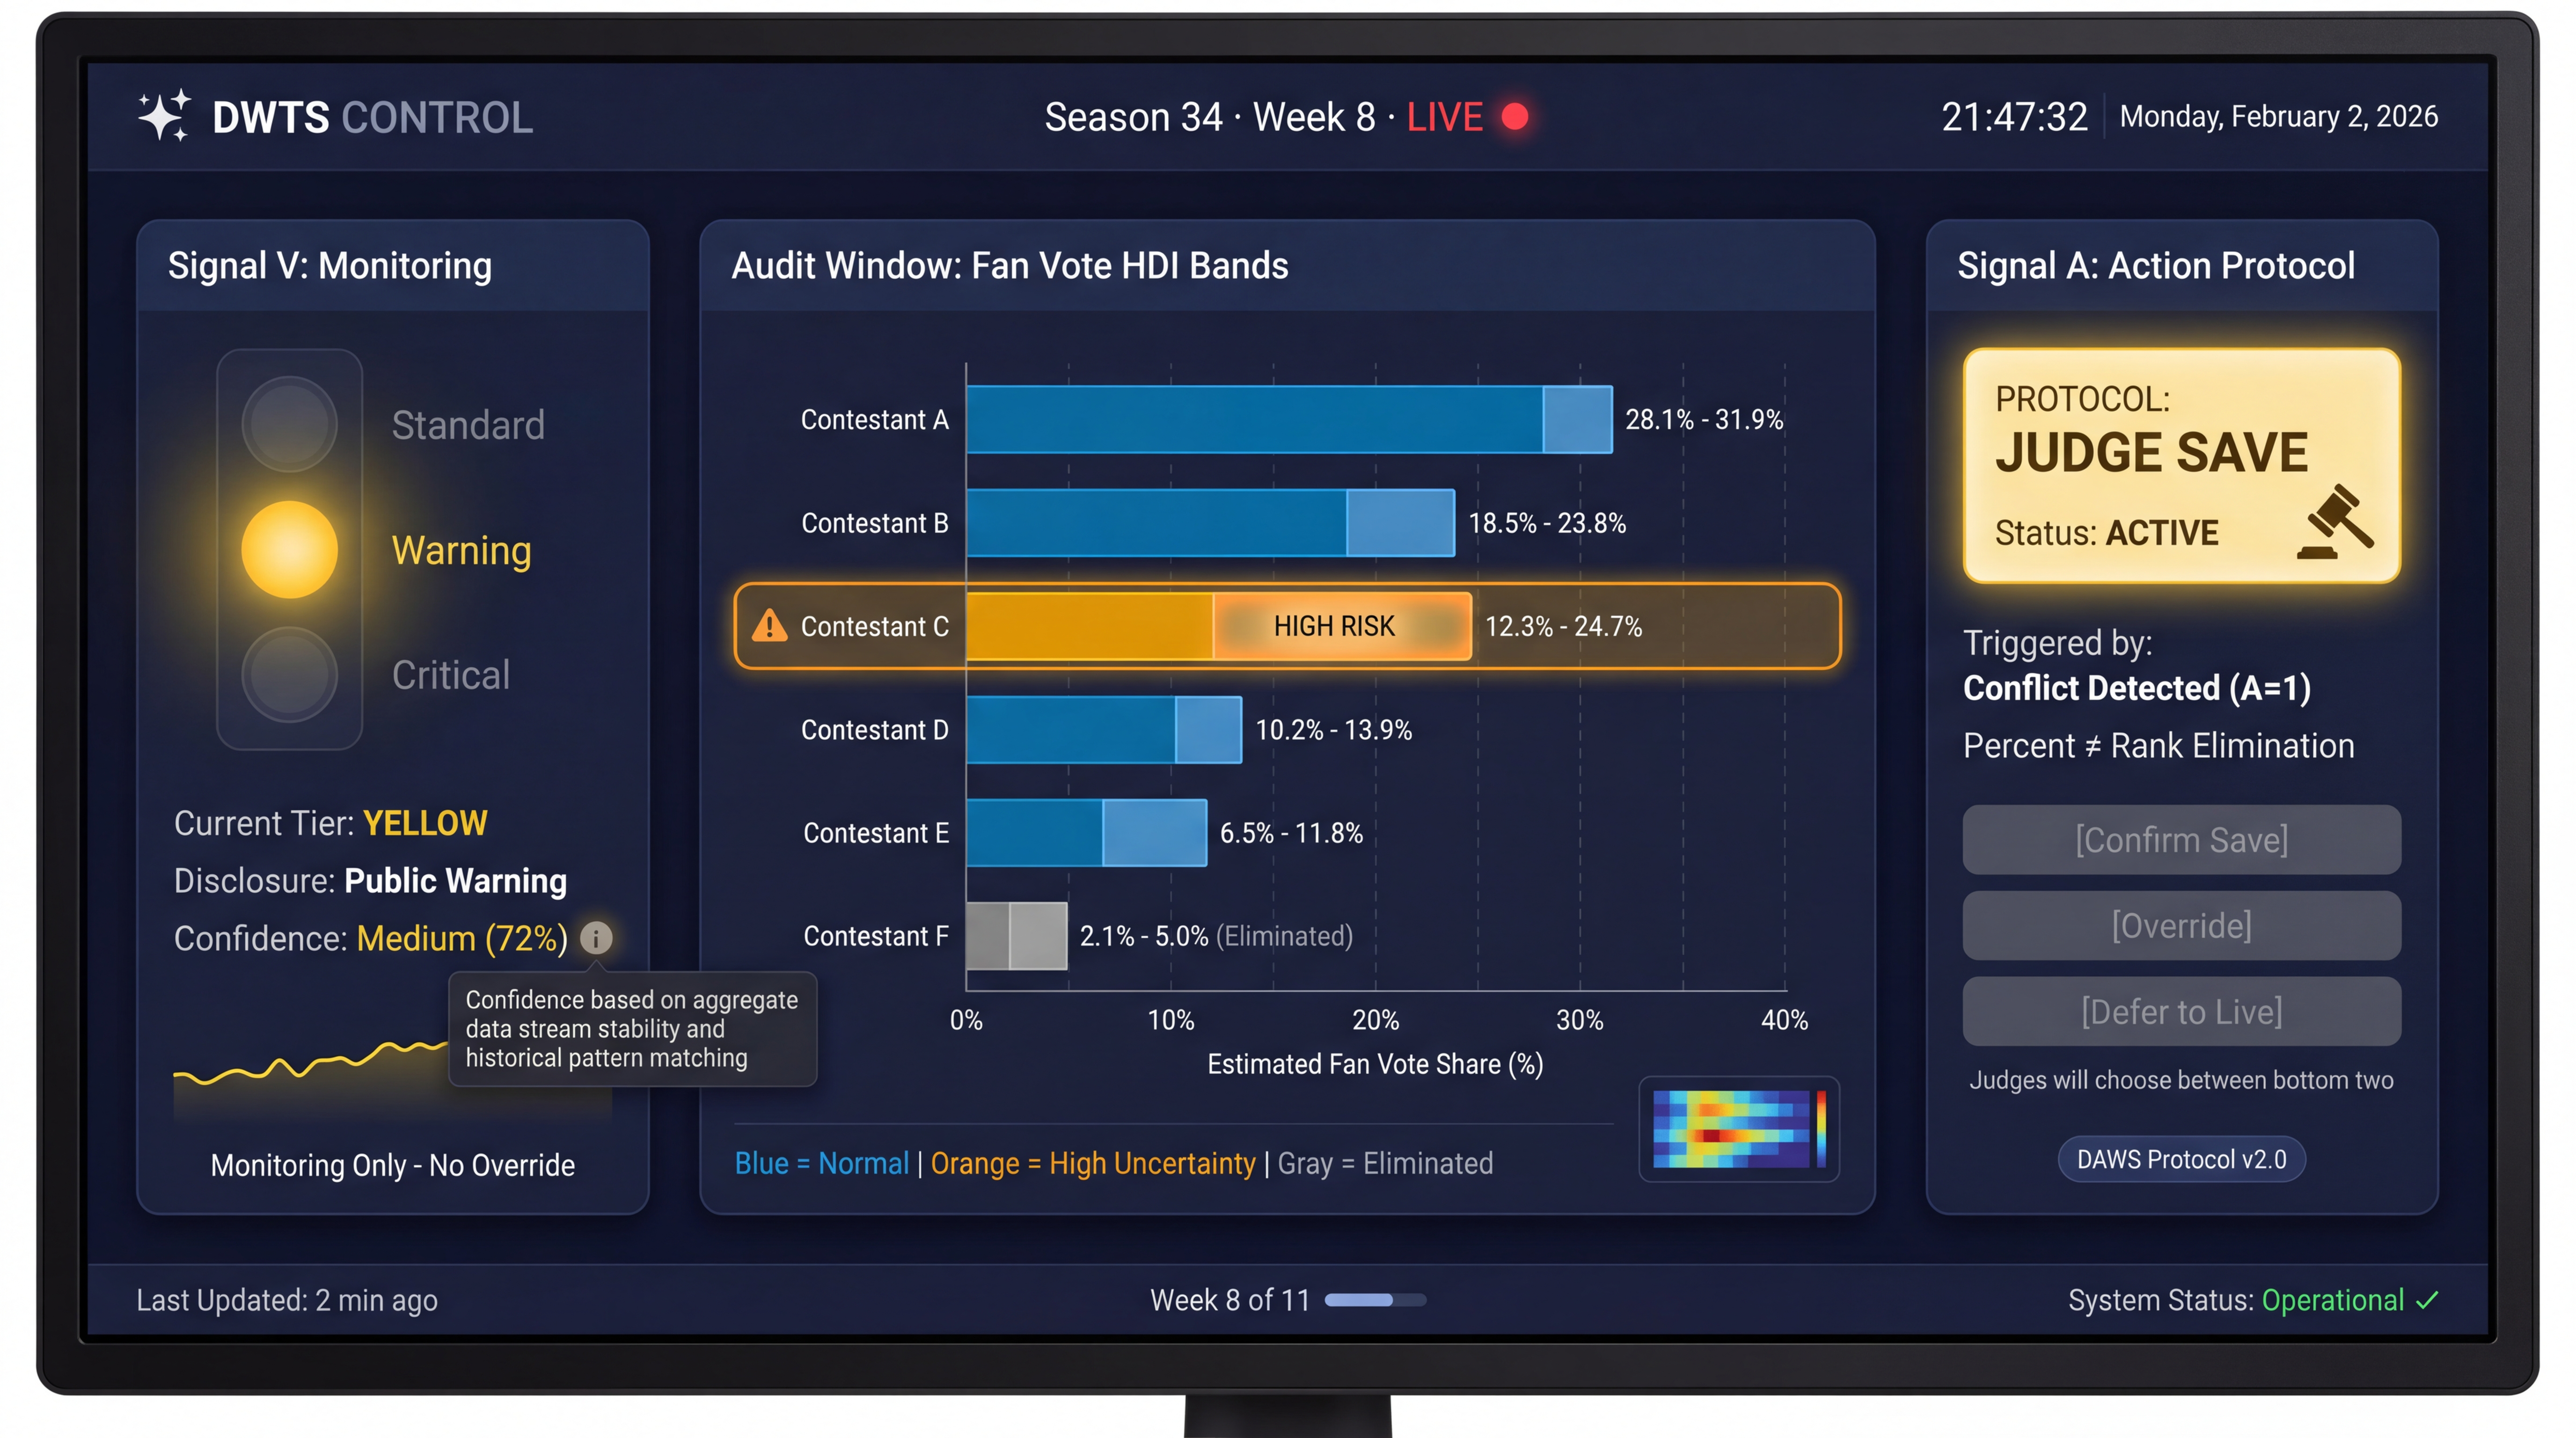
\includegraphics[width=0.98\linewidth]{figures/aigenerate/DAWS.jpg}
\caption{面向制作人的 DAWS 控制仪表板模拟:Signal V 监控等级、观众投票 HDI 审计窗口与冲突触发的评委救援协议(Signal A),呈现在可广播的决策面板中。}
\label{fig:daws-dashboard}
\end{figure}

% 机制对比雷达图
\noindent\begin{minipage}[t]{0.49\linewidth}
\centering
\includegraphics[width=\linewidth]{figures/fig_mechanism_radar.pdf}
\captionof{figure}{机制权衡(全周;指标按周聚合)。}
\end{minipage}\hfill
\begin{minipage}[t]{0.49\linewidth}
\centering
\includegraphics[width=\linewidth]{figures/fig_mechanism_radar_conflict.pdf}
\captionof{figure}{机制权衡(仅冲突周,此时百分比与排名不一致)。}
\end{minipage}

\clearpage
\addcontentsline{toc}{section}{References}
\bibliographystyle{plain}
\bibliography{ref}

\clearpage
\section*{AI 工具使用报告}
\addcontentsline{toc}{section}{AI 工具使用报告}
\noindent\textbf{披露声明。} 我们遵循 COMAP AI 政策,在下文披露所有 AI 工具的使用情况。AI 工具仅作为提高效率的辅助;所有建模选择、公式、代码逻辑与结论均由团队制定与审核,未引入竞赛数据集以外的外部数据。

\noindent\textbf{典型使用记录(简要)。} 下列条目总结了开发中使用的提示与输出。输出在被引用前均由团队审阅、编辑与核实。
\begin{enumerate}[leftmargin=2em, itemsep=0.9em]
\item \textbf{OpenAI ChatGPT}(2026 年 2 月版本,ChatGPT 5.2,Thinking 模式)。\\
\textbf{查询 1:} 设计数据加载、约束检测、采样与报告的模块化流程。\\
\textbf{输出:} 提供模块边界、建议输入/输出与调用图;我们在代码中实现并调整了该结构。\\
\textbf{查询 2:} 编写简单形上淘汰约束的严格可行性检查 Python 实现。\\
\textbf{输出:} 给出如下函数摘录(源自管线、经手动编辑与测试后):\\
\begin{verbatim}
def strict_feasible_check(
    v: np.ndarray,
    elim_idx: List[int],
    eps_sum: float = EPS_SUM,
    eps_ord: float = EPS_ORD,
) -> Tuple[bool, float, float]:
    """Strict feasible check: simplex + elimination (ties allowed)."""
    simplex_resid = float(abs(float(np.sum(v)) - 1.0))
    if len(elim_idx) == 0:
        elim_resid = 0.0
        ok = bool(simplex_resid <= eps_sum and np.all(v >= -eps_ord))
        return ok, simplex_resid, elim_resid
    n = len(v)
    elim_mask = np.zeros(n, dtype=bool)
    elim_mask[elim_idx] = True
    if np.all(elim_mask) or np.all(~elim_mask):
        elim_resid = float("nan")
        return False, simplex_resid, elim_resid
    max_e = float(np.max(v[elim_mask]))
    min_s = float(np.min(v[~elim_mask]))
    elim_resid = max_e - min_s
    ok = bool(simplex_resid <= eps_sum and np.all(v >= -eps_ord) and elim_resid <= eps_ord)
    return ok, simplex_resid, elim_resid
\end{verbatim}
\textbf{查询 3:} 针对向量化采样循环提出形状/索引错误的排查建议。\\
\textbf{输出:} 给出诊断清单(数组形状、广播规则与掩码)及向量化重写;我们在本地应用并验证了这些调整。\\
\textbf{查询 4:} 用 LaTeX 简要描述可行性审计及残差涵义。\\
\textbf{输出:} 释述简单形残差与淘汰残差的段落,后续为清晰度调整并对齐我们的符号。\\
\textbf{查询 5:} 提供采样管线(提案、过滤、汇总)的伪代码轮廓。\\
\textbf{输出:} 给出高层算法纲要;我们在 Python 中实现最终版本并验证度量。

\item \textbf{Anthropic Claude}(2026 年 2 月版本,Claude Opus 4.5)。\\
\textbf{查询 1:} 识别每周淘汰逻辑的潜在边界情形(并列、多人淘汰、缺失得分)。\\
\textbf{输出:} 提供案例清单与防护建议(并列处理、空周检查、边界条件),我们已纳入验证环节。\\
\textbf{查询 2:} 制定采样规模与评委-观众权重的敏感性分析计划。\\
\textbf{输出:} 描述逐步计划(改变种子、提案、权重,比较稳定性与翻转率),用于构建稳健性测试框架。\\
\textbf{查询 3:} 用通俗语言解释 DAWS 规则。\\
\textbf{输出:} 简洁段落说明触发周与评委救援逻辑;我们据此调整至最终术语。\\
\textbf{查询 4:} 审查百分比与排名汇总的差异以澄清歧义。\\
\textbf{输出:} 强调排名如何压缩信息并可能改变淘汰顺序的简要说明,助力我们优化措辞。

\item \textbf{Google Gemini}(2026 年 2 月版本,Gemini 3 Pro 预览)。\\
\textbf{查询 1:} 推荐最能传达不确定性与规则对比的图表类型。\\
\textbf{输出:} 建议 HDI 带、机制雷达图与稳定性对比柱;我们甄选其中部分并实施。\\
\textbf{查询 2:} 改写技术段落,降低歧义且不改变含义。\\
\textbf{输出:} 提供主语更清晰、句式更简洁的改写;团队对最终文本进行了润色。\\
\textbf{查询 3:} 简要说明后验观众份额区间的解读。\\
\textbf{输出:} 给出 3-4 句解释,先用作草稿,后调整兼容本研究符号与结果。\\
\textbf{查询 4:} 为机制折中雷达图提出简洁图注建议。\\
\textbf{输出:} 给出强调代理性、诚信与稳定性的一句话图注;我们据此调整至最终图例。

\item \textbf{Nanobananapro}(2026 年 2 月版本)。\\
\textbf{查询 1:} 利用图像识别识别图中轴、标签、图例与关键区域,以便撰写图注与检查一致性。\\
\textbf{输出:} 检出标签与元素描述;我们在采纳前与原图逐一核对。\\
\textbf{查询 2:} 检测导出图中低对比度文字或重叠注释。\\
\textbf{输出:} 列出潜在重叠与低对比区域;我们据此调整标签位置与颜色。\\
\textbf{查询 3:} 确认热图类图的轴方向与标签顺序。\\
\textbf{输出:} 提供轴标签与刻度顺序清单;我们确认与绘图数据一致。
\end{enumerate}

\noindent\textbf{验证与责任。}
\begin{itemize}[leftmargin=2em]
\item 我们审查了所有 AI 辅助产出,确保其准确、一致且相关,并修复发现的问题。
\item 我们核实 AI 输出未引入外部数据或未经支持的结论。
\item 我们检查所有引用与参考文献,确保其正确完整。
\item 团队对最终报告、代码与结论承担全部责任。
\end{itemize}

\end{document}
